%--------------------------------------------------------------------------
%	CAPITOLO 9
%---------------------------------------------------------------------------

\chapter{Le grandi firme}
Le nostre amministrazioni hanno avuto il privilegio di essere mandate alla storia per le grandi firme che le hanno assunte.
Infatti leggiamo\footnote{Anticipo ai lettori che le firme sopracitate, sono appartenenti ai personaggi di una certa importanza che sbagliavano a scrivere il proprio nome, o lo facevano in modo incomprensibile. Mingazzi ha riportato le firme erronee degli assessori \textbf{Fagioli Angelo}, \textbf{Natali Alessandro} e dei consiglieri comunali \textbf{Poletti Raffaele} e \textbf{Garavini Battista}}:

\begin{center}
	\Huge
	\textcal{L'Assessore \hspace{2.5cm} L'Assessore}
	\normalsize
	\footnote{\textbf{Natali Alessandro}, un assessore supplente nella giunta comunale del 1902, con \index[Personaggi]{Alberani Alberto}Alberani Alberto sindaco. Faceva parte dei clericali. Viveva nell'edificio dove c'era il \index[Luoghi]{Teatro Camerani}Teatro Camerani nella \index[Luoghi]{Violina (via)}Violina e l'aveva trasformato in una fabbrica di paste alimentari. Fin dai primi del '900 svolgeva questa attività, con i figli Pietro e Giacomo Natali.\index[Personaggi]{Natali Pietro}\index[Personaggi]{Natali Giacomo}}
\end{center}
	
 \begin{figure}[htb]
    \vspace{-0.75cm}
    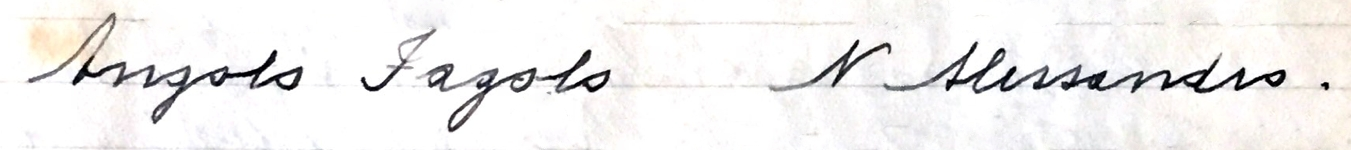
\includegraphics[width=\textwidth]{firme1}
    \caption[Firme]{\label{fig:firme1}}
    \vspace{-1cm}
\end{figure}\index[Personaggi]{Angelo Fagioli (assessore)}
\index[Personaggi]{Natali Alessandro (assessore)}

\begin{center}
	\Huge
	\textcal{Il membro della Cong. Carità}
	\normalfont
	\normalsize
	\footnote{\textbf{Congregazione di carità} è la denominazione ottocentesca delle istituzioni statali destinate a venir incontro ai bisogni della popolazione povera. Era legata all'\index[Luoghi]{Ospedale G. Gamberini di Alfonsine}Ospedale G. Gamberini di Alfonsine e ne gestiva le donazioni.}
\end{center}

\begin{figure}[htb]
    \centering
    \vspace{-0.65cm}
    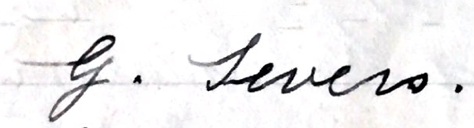
\includegraphics[width=0.45\textwidth]{firme2}
    \caption*{\label{fig:firme2}}
    \vspace{-0.3cm}
\end{figure}
\index[Personaggi]{G. Severo}

\normalfont
\vspace{2cm}

\indent Vi erano poi anche ai margini delle amministrazioni altre firme di valore:
	
	\begin{figure}[htb]
	    \centering
	    \vspace{-0.4cm}
	    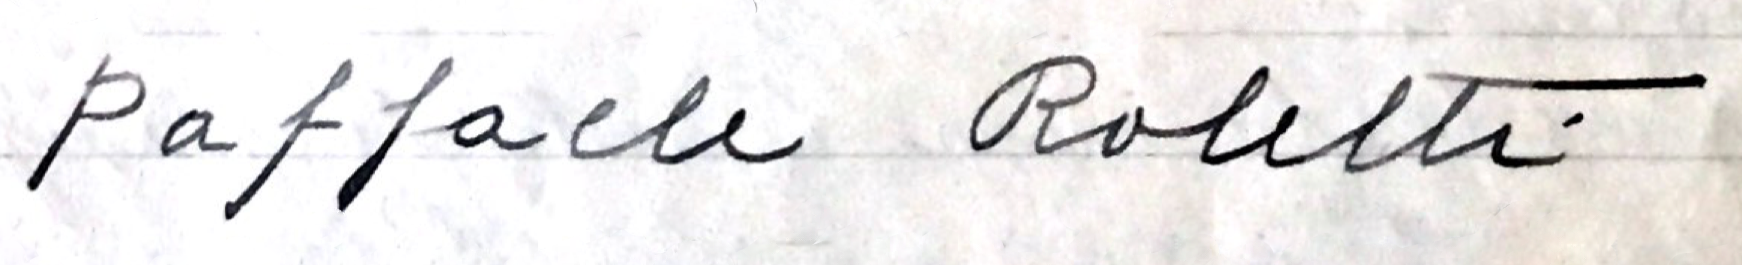
\includegraphics[width=0.8\textwidth]{firme3}
	    \caption*{\label{fig:firme3}}
	    \vspace{-0.7cm}
	\end{figure}
	
\index[Personaggi]{Poletti Raffaele (consigliere comunale)}

firma che valeva molto su di una cambiale\footnote{Nel diritto italiano, è un titolo di credito la cui funzione tipica è quella di rimandare il pagamento di una somma in denaro.} anche perché l'artefice prima di stamparla aveva bisogno di provare molte paia di occhiali, poi accusava di non trovarne un paio adatti, poi la penna si spuntava, la carta si forava, l'inchiostro macchiava, non scorreva, mezz'ora prendeva la posizione adatta, e racconti della caduta del papa tra una sillaba e l'altra, quella della cacciata dei carabinieri del papa ecc. ecc. e finalmente dalle 9 alle 12 poteva uscire la gran firma. \\

\indent Altra firma era

	\begin{figure}[htb]
	    \centering
	    \vspace{-0.3cm}
	    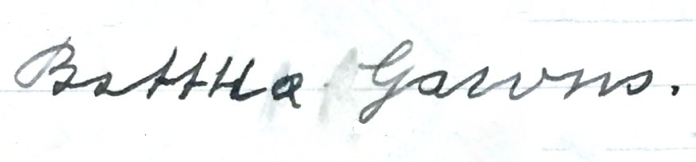
\includegraphics[width=0.7\textwidth]{firme4}
	    
	    \caption*{\label{fig:firme4}}
	    \vspace{-1.6cm}
	\end{figure}\footnote{Potrebbe trattarsi di \textbf{Battista Garavini}\index[Personaggi]{Garavini Battista (agente municipale)}, che fu un agente municipale  e protocollista attorno al 1810. Una curiosità: nel 1831, durante i moti, una folla di cittadini si presentò a casa del gonfaloniere \index[Personaggi]{Corelli Giuseppe (gonfaloniere)}Giuseppe Corelli, chiedendo che venisse dimesso il cancelliere,  e tra altre persone, anche l'impiegato Garavini\index[Personaggi]{Garavini Battista (agente municipale)}. Le motivazioni di queste richieste sono confuse: "per l'impudenza, l'alterigia, la troppa lingua, la sfacciataggine e non riconoscenza." come riportò Corelli.}

	
\indent gerente responsabile di bellissimi articoli polemici paesani sul Corriere di Romagna.



